\chapter{Background}
\label{ch:background}
\glsresetall
Having introduced the subject of this Master Thesis in the previous chapter (by means of answers to important ``Wh''-questions), this chapter dives deeper into the background concepts that this research builds upon. Specifically, this chapter aims to answer the following questions:
\begin{fullwidth}
    \begin{itemize}
        \item What is the Transformer architecture in general and BERT specifically?
        \item What is Knowledge Distillation?
        \item How do we evaluate our approach?
    \end{itemize}
\end{fullwidth}
    
To this end, this chapter first introduces the \gls{seq2seq} architecture in \cref{sec:seq2seq_architectures}, which has brought about significant advances in transduction tasks, such as translation, question answering and speech recognition, among others. The original or ``conventional'' \gls{seq2seq} architecture relies on recurrence to compute representations of its input and output, which does come with certain drawbacks, however. As such, an important improvement of the conventional \gls{seq2seq} architecture is introduced next, which relies on attention mechanisms.

Next, the inner workings of the \emph{Transformer} architecture are detailed in \cref{sec:transformer_architecture}. As a deeper, attention-only \gls{seq2seq} architecture, it has been responsible for a recent wave of advancements in the domains of \gls{nlu} and \gls{nlg}. 

Third, the \bertbase architecture is reviewed in \cref{sec:bert}, highlighting the differences between it and the original Transformer architecture. As mentioned previously in \cref{ch:introduction}, this is the particular Transformer-based architecture used in the current research. 

Penultimately, \cref{sec:knowledge_distillation} introduces \gls{kd}, a \gls{nn} compression method that has gained popularity in recent years, especially when it comes to Transformer(-based) architectures (see \cref{ch:related_work}). Again, as introduced in the previous chapter, this is the particular \gls{nn} compression method under investigation in this research.

Finally, \cref{sec:evaluation} presents the methods with which our approach will be evaluated in the present work. Specifically, we'll first detail the \gls{glue} benchmark, a collection of 9 \gls{nlu} tasks (with accompanying datasets), before introducing the \gls{squad}, a sizable reading comprehension dataset.



\section{Sequence-to-sequence Architectures}
\label{sec:seq2seq_architectures}
\glsreset{seq2seq}

\subsection{Conventional sequence-to-sequence architectures}

Originally developed for the purposes of \gls{nmt}, conventional \gls{seq2seq} \gls{nn} architectures \citep{sutskever2014sequence,cho2014learning} rely on \glspl{rnn} to compute representations of their input and output. These \glspl{nn} are composed of an \emph{encoder}, which encodes an input (or ``source'') sequence into a fixed-length vector (often called a ``context'' or ``thought'' vector), and a \emph{decoder}, which uses this encoded vector to compute the output (or ``target'') sequence, as illustrated in \cref{fig:seq2seq_model_architecture}.

\begin{figure}[ht!]
    \centering
    % \def\svgwidth{0.75\linewidth}
    \def\svgscale{0.8}
    \includesvg{figures/04-background/seq2seq-details}
    % 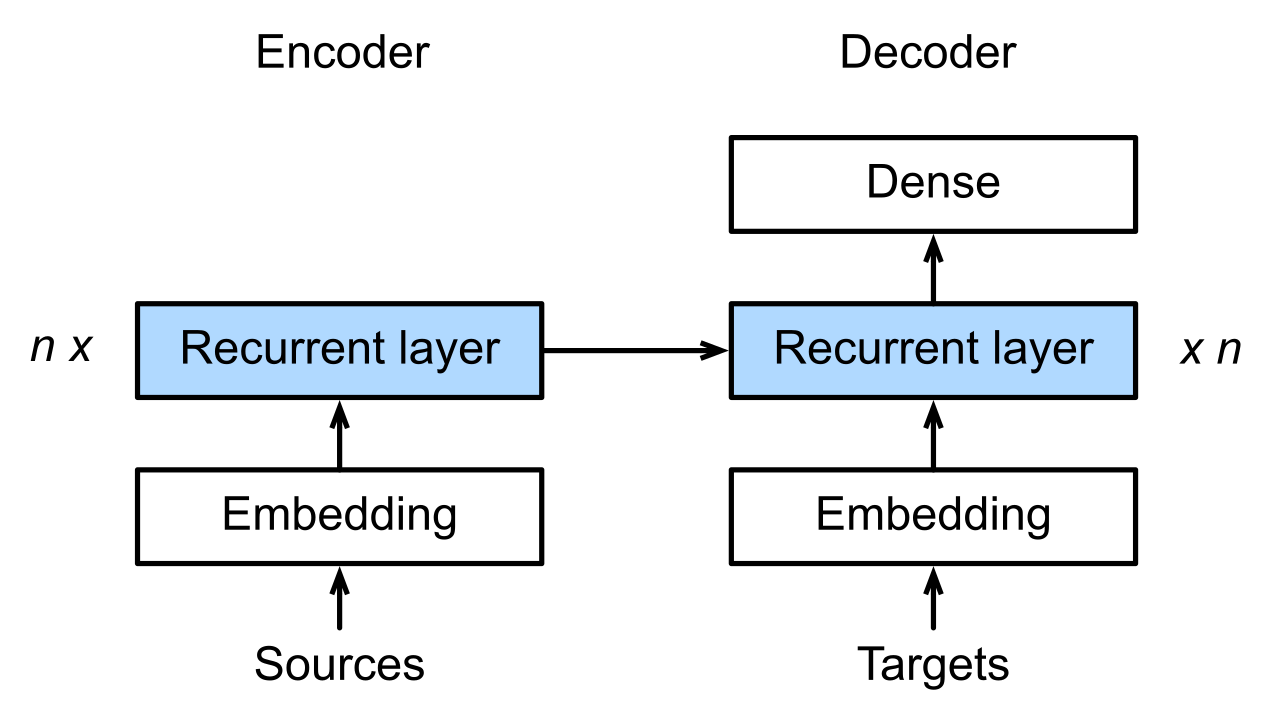
\includegraphics[width=\linewidth]{figures/04-background/seq2seq-details.png}
    \caption[The seq2seq network architecture]{The sequence-to-sequence network architecture. Source: \href{https://d2l.ai/chapter_recurrent-modern/seq2seq.html}{Dive into Deep Learning}}
    \label{fig:seq2seq_model_architecture}
\end{figure}

Formally, given an input sequence $\xvect = \begin{bmatrix} \xvect_1 & \xvect_2 & \cdots & \xvect_N \end{bmatrix}^{\top}$ of length $N$, the encoder of conventional \gls{seq2seq} networks encodes this input sequence $\xvect$ into a context vector $\cvect$ of length $M$ as follows:
\begin{align}
    \hvect_i &= f(\xvect_i, \hvect_{i-1}), \\
    \cvect &= q(\begin{Bmatrix} \hvect_1, & \hvect_2, & \cdots, & \hvect_N \end{Bmatrix}),
\end{align}

where $\hvect_n \in \reals{M}$ is the hidden state of the encoder at step $t$ and $f$ and $q$ are some non-linear functions. For example, \citet{sutskever2014sequence} use
\begin{align*}
    \hvect_i &= f(\xvect_i, \hvect_{i-1}) = \text{LSTM}(\xvect_i, \hvect_{i-1}), \\
    \cvect &= q(\begin{Bmatrix} \hvect_1, & \hvect_2, & \cdots, & \hvect_N \end{Bmatrix}) = \hvect_N,
\end{align*}

where $\text{LSTM}$ is the \emph{\glsdesc{lstm}} \citep{hochreiter1997long}. 

The decoder now uses this context vector $\cvect$ and any previously predicted elements of the output sequence $\begin{Bmatrix} y_1, & y_2, & \cdots, & y_{t-1} \end{Bmatrix}$ to predict the next element of the output sequence $y_{t}$. This joint probability is given by:
\begin{align}
    \label{eq:prod_conditional_probabilities}
    p(\yvect) = \prod_{t=1}^{T} p\left(y_{t} | \cvect, \begin{Bmatrix} y_1, & y_2, & \cdots, & y_{t-1} \end{Bmatrix} \right),
\end{align}

where $\yvect = \begin{bmatrix} y_1 & y_2 & \cdots & y_{T} \end{bmatrix}^{\top}$ is the output sequence of length $T$. Again using an \gls{rnn} for the decoder, the hidden state $\svect_{t}$ of the decoder is given by:
\begin{align}
    \label{eq:conventional_decoder_hidden_state}
    \svect_{t} &= f(\cvect, y_{t-1}, \svect_{t-1}), \\
    \svect_{t=0} &= \hvect_N,
\end{align}

where $f$ is the same non-linear function as used for the encoder, and the hidden state of the encoder at the last step $\hvect_N$ is used as the initial hidden state of the decoder $\svect_{t=0}$. As such, we can compute the conditional probabilities in \cref{eq:prod_conditional_probabilities} as follows:
\begin{align}
    \label{eq:conventional_conditional_probability}
    p\left( y_{t} | \cvect, \begin{Bmatrix} y_1, & y_2, & \cdots, & y_{t-1} \end{Bmatrix} \right) = g(\cvect, y_{t-1}, \svect_{t}),
\end{align}

where $g$ is again some non-linear function.


\subsection{Sequence-to-sequence architectures with attention}

While these conventional \gls{seq2seq} models perform well for relatively short sequences, they do suffer from deteriorating performance as the length of the sequence increases \citep{cho2014properties}. To address this issue, attention mechanisms were introduced as an extension to the conventional encoder-decoder architecture \citep{bahdanau2014neural,luong2015effective}, as illustrated in \cref{fig:seq2seq_with_attention_model_architecture}, which significantly outperform their conventional counterparts, regardless of the sequence length.

\begin{figure}[ht!]
    \centering
    % \def\svgwidth{\linewidth}
    \def\svgscale{0.8}
    \includesvg{figures/04-background/seq2seq-attention-details}
    % 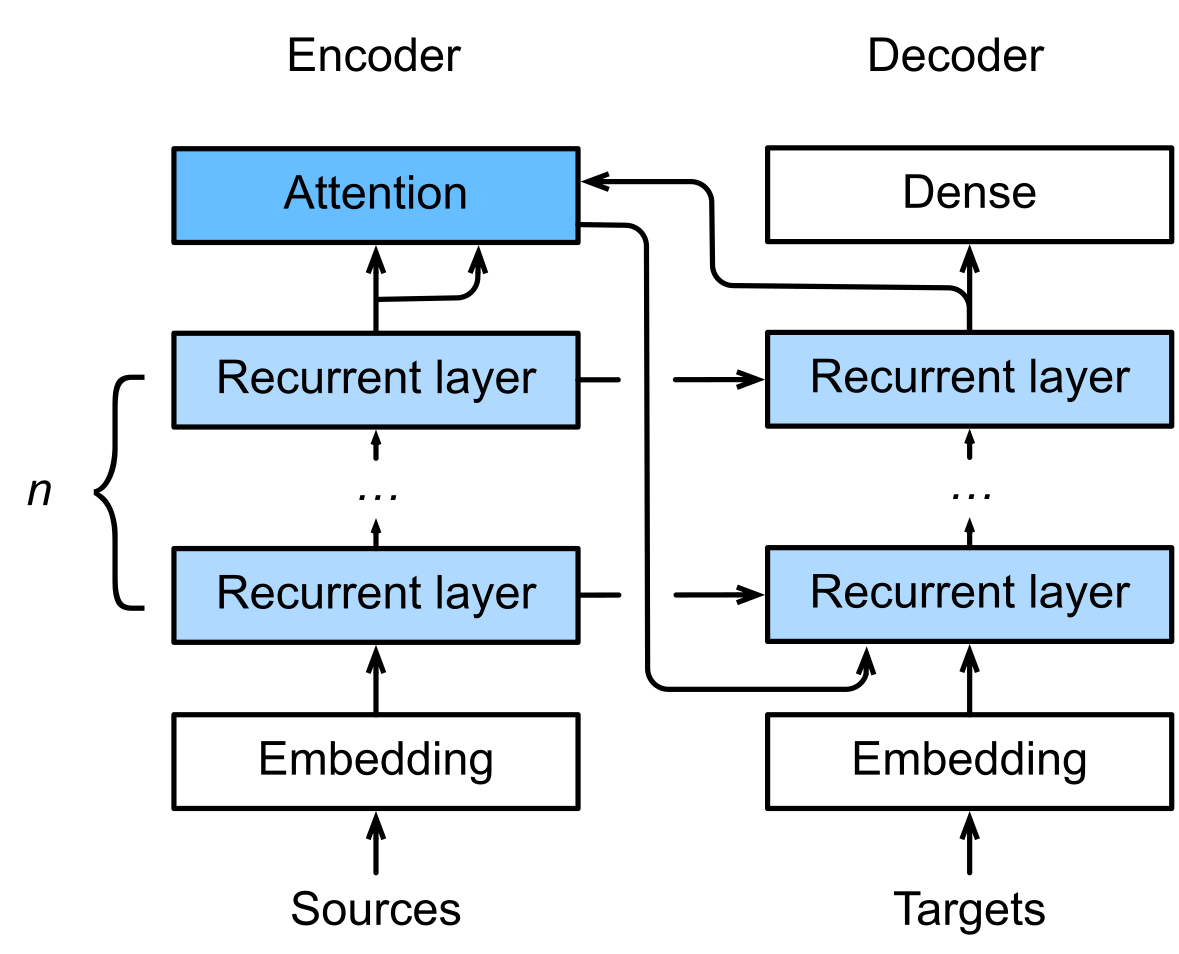
\includegraphics[width=\linewidth]{figures/04-background/seq2seq-attention-details.png}
    \caption[The seq2seq network architecture with attention mechanisms]{The sequence-to-sequence network architecture with attention mechanisms. Source: \href{https://d2l.ai/chapter_attention-mechanisms/bahdanau-attention.html}{Dive into Deep Learning}}
    \label{fig:seq2seq_with_attention_model_architecture}
\end{figure}

Instead of using a single fixed-length context vector $\cvect$ as an encoding for the entire input sequence, these \gls{seq2seq} models with attention mechanism(s) use a (variable length) sequence of context vectors for the encoding instead. Whenever the decoder generates a new element of the output sequence, it soft-searches for the most informative elements in the input sequence, and then uses the context vectors associated with these most informative elements and all previously generated output elements as input.

As such, \cref{eq:conventional_decoder_hidden_state,eq:conventional_conditional_probability} can be updated as follows:

\begin{align}
    \svect_t &= f(\cvect_t, y_{t-1}, \svect_{t-1}), \\
    \label{eq:attentative_conditional_probability}
    p\left( y_t | \xvect, \begin{Bmatrix} y_1, & y_2, & \cdots, & y_{t-1} \end{Bmatrix} \right) &= g(\cvect_t, y_{t-1}, \svect_t),
\end{align}

where for each element of the output sequence $y_t$, $\cvect_t$ is a distinct context vector which depends on all hidden states of the encoder $\begin{Bmatrix} \hvect_1, & \hvect_2, & \cdots, & \hvect_N \end{Bmatrix}$ as follows:

\begin{align}
    \label{eq:context_vector_weighted_sum}
    \cvect_t &= \sum_{i=1}^{N} \alpha_{t,i} \hvect_i,
\end{align}

where $\alpha_{t,i}$ serves as a weight of each encoder hidden state $\hvect_i$

\begin{align}
    \label{eq:softmax_scoring_function}
    \alpha_{t,i} &= \frac{\expp{\scoree{\svect_{t-1}, \hvect_i}}}{\sum_{i'=1}^N \expp{\scoree{\svect_{t-1}, \hvect_{i'}}}}.
\end{align}

In fact, $\alpha_{t,:}$ describes a probability distribution over the $N$ encoder hidden states $\begin{Bmatrix} \hvect_1, & \hvect_2, & \cdots, & \hvect_N \end{Bmatrix}$ using the softmax function over the \emph{alignment score} between decoder hidden state $\svect_{t-1}$ and encoder hidden state $\hvect_i$. Here, \citet{bahdanau2014neural} parameterize this alignment score function as a simple \gls{ffn}, which is trained jointly with the encoder and decoder:

\begin{align}
    \label{eq:bahdanau_scoring_function}
    \scoree{\svect_{t-1}, \hvect_i} &= \vect{V}_{\alpha}^{\top} \tanhh{\Wvect_{\alpha} \left[ \svect_{t-1}; \hvect_i \right]},
\end{align}

where $\vect{V}_{\alpha} \in \reals{M}$, $\Wvect_{\alpha} \in \reals{M \times 2M}$ are learnable weight matrices.\sidenote{Actually, \citet{bahdanau2014neural} use a \gls{birnn} for the encoder, such that every encoder hidden state $\hvect_i$ is a concatenation of the hidden state $\overrightarrow{\hvect_i}$ of the forward \gls{rnn} $\overrightarrow{f}$ and the hidden state $\overleftarrow{\hvect_i}$ of the backward \gls{rnn} $\overleftarrow{f}$: \begin{align*}\hvect_i = \left[ \overrightarrow{\hvect_i}; \overleftarrow{\hvect_i} \right].\end{align*} \\ As such, the alignment score in \cref{eq:bahdanau_scoring_function} should actually be:
\begin{align*}\scoree{\svect_{t-1}, \hvect_i} &= \vect{V}_{\alpha}^{\top} \tanhh{\Wvect_{\alpha} \svect_{t-1} + \vect{U}_{\alpha} \hvect_i},\end{align*} where $\vect{V}_{\alpha} \in \reals{M}$, $\Wvect_{\alpha} \in \reals{M \times M}$ and $\vect{U}_{\alpha} \in \reals{M \times 2M}$ are learnable weight matrices.}


% \subsection{seq2seq network architectures with convolution}
% Another drawback of these conventional \gls{seq2seq} models is that they are inherently sequential in nature, as the hidden state $\hvect_i$ is a function of the input for position $i$ and the previous hidden state $\hvect_{i-1}$. Especially for longer sequence lengths this becomes problematic, as its sequential nature does not allow for the parallel computation of these hidden states within a sequence. To address this concern, \glspl{cnn} were introduced as a replacement for \glspl{rnn} in the encoder-decoder architecture \citep{kalchbrenner2016neural,gehring2017convolutional}. These \gls{cnn}-based architectures do allow for parallelization over every element in a sequence, making them an order of magnitude faster than conventional \gls{seq2seq} \glspl{nn}.



\section{Transformer Architecture}
\label{sec:transformer_architecture}

Even though \gls{seq2seq} architectures with attention mechanisms outperform their conventional counterparts (especially for longer sequences), they still rely on recurrence to compute representations of their input and output. This makes them inherently sequential in nature, as the hidden state $\hvect_i$ is still a function of the input for position $i$ and the previous hidden state $\hvect_{i-1}$. Their sequential nature disallows for parallel computation of these hidden states, making their run time super-linear in the length of the input and target sequence \citep{kalchbrenner2016neural,gehring2017convolutional}.

The \emph{Transformer} architecture \citep{vaswani2017attention} addresses this drawback by completely dispensing with recurrence altogether, instead relying entirely on (self-)attention mechanisms to compute representations of the input and output sequences. It does so by using encoder and decoder stacks, which are both comprised of stacked self-attention and position-wise fully connected layers, as illustrated in \cref{fig:transformer_model_architecture}. In the following subsections, all components of the Transformer architecture will be explained in detail.

\begin{figure}[ht!]
    \centering
    % \def\svgwidth{\linewidth}
    \def\svgscale{0.8}
    \includesvg{figures/04-background/transformer}
    % 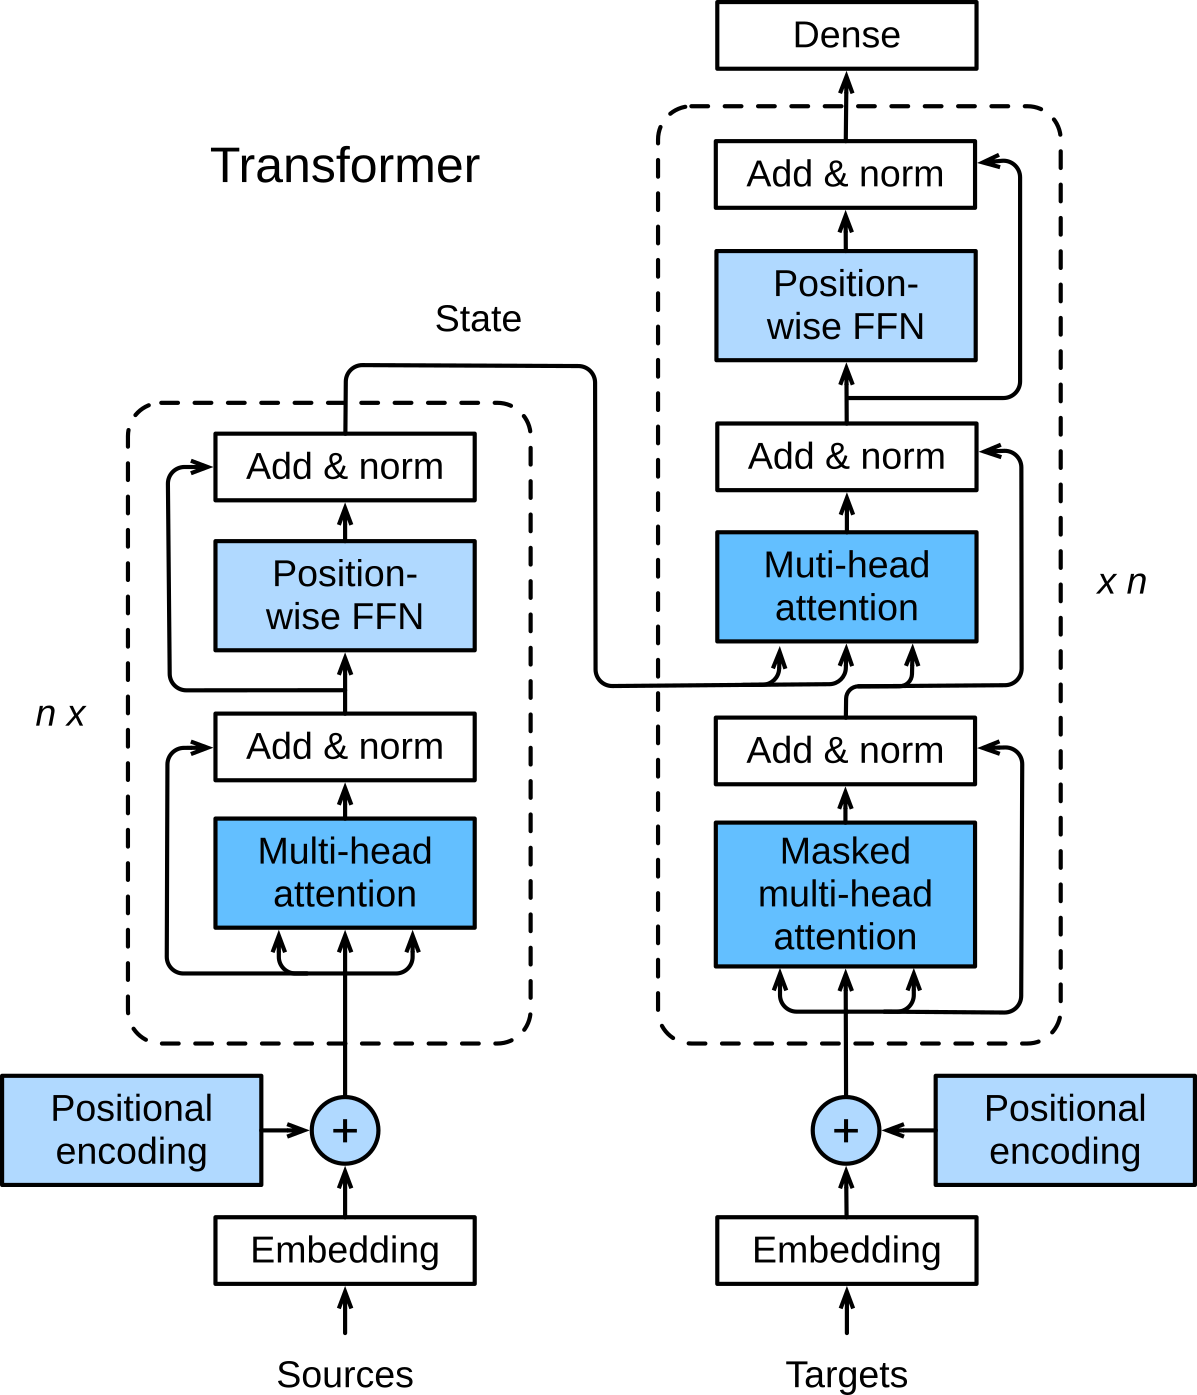
\includegraphics[width=\linewidth]{figures/04-background/transformer.png}
    \caption[The Transformer network architecture]{The Transformer network architecture. Source: \href{https://d2l.ai/chapter_attention-mechanisms/transformer.html}{Dive into Deep Learning}}
    \label{fig:transformer_model_architecture}
\end{figure}

\subsection{Encoder and Decoder}
\label{subsec:encoder_decoder}

\subsubsection{Encoder}
\label{subsubsec:encoder}
The encoder stack consists of $N = 6$ (identical) layers, with two sub-layers each. The first sub-layer is a multi-head attention layer, and the second is a position-wise \gls{ffn}. Both sub-layers have residual connections around them, followed by layer normalization. All outputs of the embedding layers and sub-layers in the model are of dimension $d_{\text{model}} = 512$.

\subsubsection{Decoder}
\label{subsubsec:decoder}
Similarly, the decoder stack also consists of $N = 6$ (identical) layers, although now with three sub-layers each. The first sub-layer is a masked multi-head attention layer, such that positions in the output sequence are prevented from attending to subsequent positions. The second sub-layer is a multi-head attention layer over the output of the encoder stack. Finally, the third sub-layer is again a position-wise \gls{ffn}. As with the encoder, all sub-layers feature residual connections, followed by layer normalization.

\subsection{Attention}
\label{subsec:attention}

\subsubsection{Scaled Dot-Product Attention}
\label{subsubsec:scaled_dot_product_attention}
\citet{vaswani2017attention} introduce a new form of attention called \emph{scaled dot-product attention} that is highly similar to the \emph{dot-product attention} of \citet{luong2015effective}. In their definition, they use the $(query, key, value)$ triplet representation, where the keys and values correspond with the encoder hidden state $\hvect_i$ and the query corresponds with the decoder hidden state $\svect_{t-1}$. Now, formally, the alignment scoring function is defined as a scaled dot-product:
\begin{align}
    \scoree{\vect{q}, \vect{k}} &= \frac{\vect{q}^{\top} \vect{k}}{\sqrt{d_k}},
\end{align}

where $d_k$ is the dimension of the keys. In terms of the encoder hidden state $\hvect_i$ and the decoder hidden state $\svect_{t-1}$, we get:
\begin{align}
    \label{eq:scaled_dot_product_scoring_function}
    \scoree{\svect_{t-1}, \hvect_i} &= \frac{\svect_{t-1}^{\top} \hvect_i}{\sqrt{N}},
\end{align}

where $N$ is the number of encoder hidden states $\begin{Bmatrix} \hvect_1, & \hvect_2, & \cdots, & \hvect_N \end{Bmatrix}$. This alternative scoring function can then be plugged into \cref{eq:softmax_scoring_function} to compute the context vector $\cvect_i$ using \cref{eq:context_vector_weighted_sum}.

In practice, however, all queries are packed together into a matrix $\vect{Q}$. Similarly, the keys and values are also packed together into matrices $\vect{K}$ and $\vect{V}$, respectively. The matrix of context vectors $\vect{C}$ is then given by:
\begin{align}
    \vect{C} &=  \text{Attention}\left( \vect{Q}, \vect{K}, \vect{V} \right) = \text{softmax}\left( \frac{\vect{Q} \vect{K}^{\top}}{\sqrt{d_k}} \right) \vect{V}.
\end{align}

Similarly, stacking the encoder hidden states  $\begin{Bmatrix} \hvect_1, & \hvect_2, & \cdots, & \hvect_N \end{Bmatrix}$ into a matrix $\vect{H}$ and the decoder hidden states  $\begin{Bmatrix} \svect_1, & \svect_2, & \cdots, & \svect_{t-1} \end{Bmatrix}$ into a matrix $\vect{S}$, we get:
\begin{align}
    \vect{C} &= \text{softmax}\left( \frac{\vect{S} \vect{H}^{\top}}{\sqrt{N}} \right) \vect{H}.
\end{align}

\subsubsection{Multi-Head Attention}
\label{subsubsec:multi_head_attention}

\citet{vaswani2017attention} found it beneficial to linearly project the queries, keys and values $h$ times using different, learned linear projections to $d_k$, $d_k$, and $d_v$, respectively, instead of performing a single attention function with $d_{\text{model}}$-dimensional queries, keys and values. The attention function is then applied in parallel on each of these projections, which yield $d_v$-dimensional output values. Finally, these are concatenated and projected once again in order to come to the final values, as illustrated in \cref{fig:multi-head_attention}.

\begin{figure}[ht!]
    \centering
    % \def\svgwidth{\linewidth}
    \def\svgscale{0.8}
    \includesvg{figures/04-background/multi-head-attention}
    % 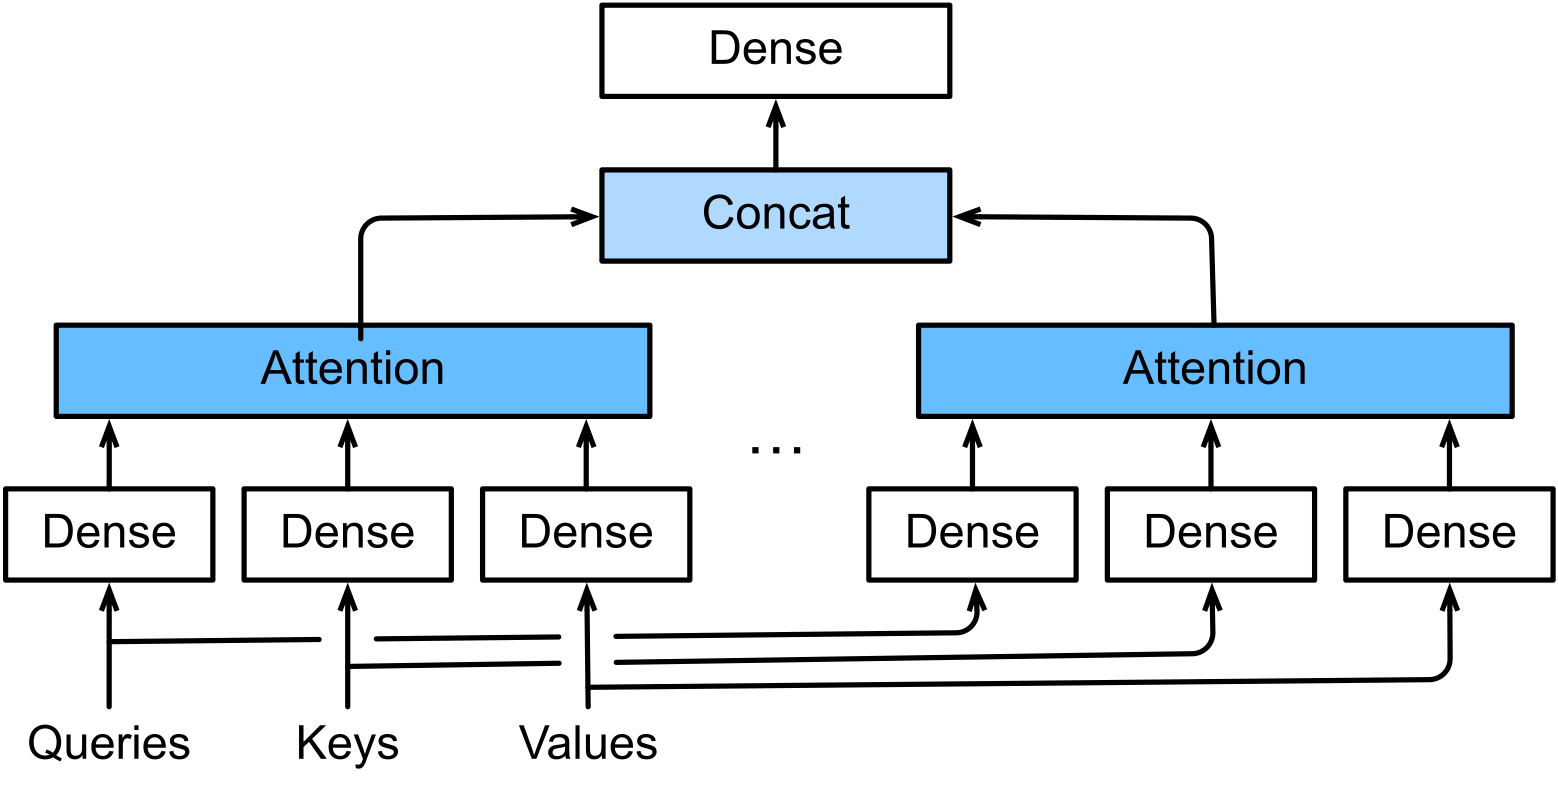
\includegraphics[width=\linewidth]{figures/04-background/multi-head-attention.png}
    \caption[Multi-Head Attention]{Multi-Head Attention. Source: \href{https://d2l.ai/chapter_attention-mechanisms/multihead-attention.html}{Dive into Deep Learning}}
    \label{fig:multi-head_attention}
\end{figure}

Formally, we have:
\begin{align}
    \text{MultiHead}\left( \vect{Q}, \vect{K}, \vect{V} \right) &= \begin{bmatrix}\text{head}_1; & \text{head}_2; & \cdots & \text{head}_h\end{bmatrix} \Wvect^O,
\end{align}

where

\begin{align}
    \text{head}_i &= \text{Attention}\left( \vect{Q} \Wvect_i^Q, \vect{K} \Wvect_i^K, \vect{V} \Wvect_i^V \right),
\end{align}

and where

\begin{align*}
    \Wvect_i^Q &\in \reals{d_{\text{model}} \times d_k}, \\
    \Wvect_i^K  &\in \reals{d_{\text{model}} \times d_k}, \\
    \Wvect_i^V  &\in \reals{d_{\text{model}} \times d_v}, \\
    \text{and } \Wvect^O &\in \reals{h d_v \times d_{\text{model}}}
\end{align*}

are the projection matrices. \citet{vaswani2017attention} use $h = 8$ attention heads with $d_k = d_v = d_{\text{model}} / h = 64$.

\subsection{Position-wise Feed-Forward Networks}
\label{subsec:position_wise_ffn}
The position-wise \gls{ffn} present in each encoder and decoder layer has only a single hidden layer, coupled with a \gls{relu} activation:

\begin{align}
    \text{FFN}(\xvect) &= \max\left( 0, \xvect \Wvect_1 + \vect{b}_1 \right) \Wvect_2 + \vect{b}_2,
\end{align}

where 

\begin{align*}
    \Wvect_1 &\in \reals{d_{\text{model}} \times d_{ff}}, \\
    \vect{b}_1 &\in \reals{d_{ff}}, \\
    \Wvect_2 &\in \reals{d_{ff} \times d_{\text{model}}}, \\
    \text{and } \vect{b}_2 &\in \reals{d_{\text{model}}}.
\end{align*}

The linear transformations use different parameters for each layer, but are applied the same across different positions. \citet{vaswani2017attention} use $d_{ff} = 2048$.

\subsection{Embeddings}
\label{subsec:embeddings}
For both the input and output sequences, \citet{vaswani2017attention} use learned embeddings to convert their elements into vectors of dimension $d_{\text{model}}$, such that a sequence vector $\vect{z} = \begin{bmatrix}z_1 & z_2 & \cdots & z_l\end{bmatrix} \in \reals{l}$ becomes a sequence embedding matrix $\vect{Z} \in \reals{l \times d_{\text{model}}}$.

\subsection{Positional Encoding}
\label{subsec:positional_encoding}
In order to preserve information about the relative or absolute position of elements in the input and output sequences, \citet{vaswani2017attention} add fixed (i.e. not learned) \emph{positional encodings} to the embeddings of the sequences, as illustrated in \cref{fig:positional_encoding}. The positional encodings have the same dimension $d_{\text{model}}$ as the embeddings, such that the two can be summed.

\begin{figure*}[ht!]
    \centering
    % \def\svgwidth{\linewidth}
    \def\svgscale{0.8}
    \includesvg{figures/04-background/positional-encoding}
    % 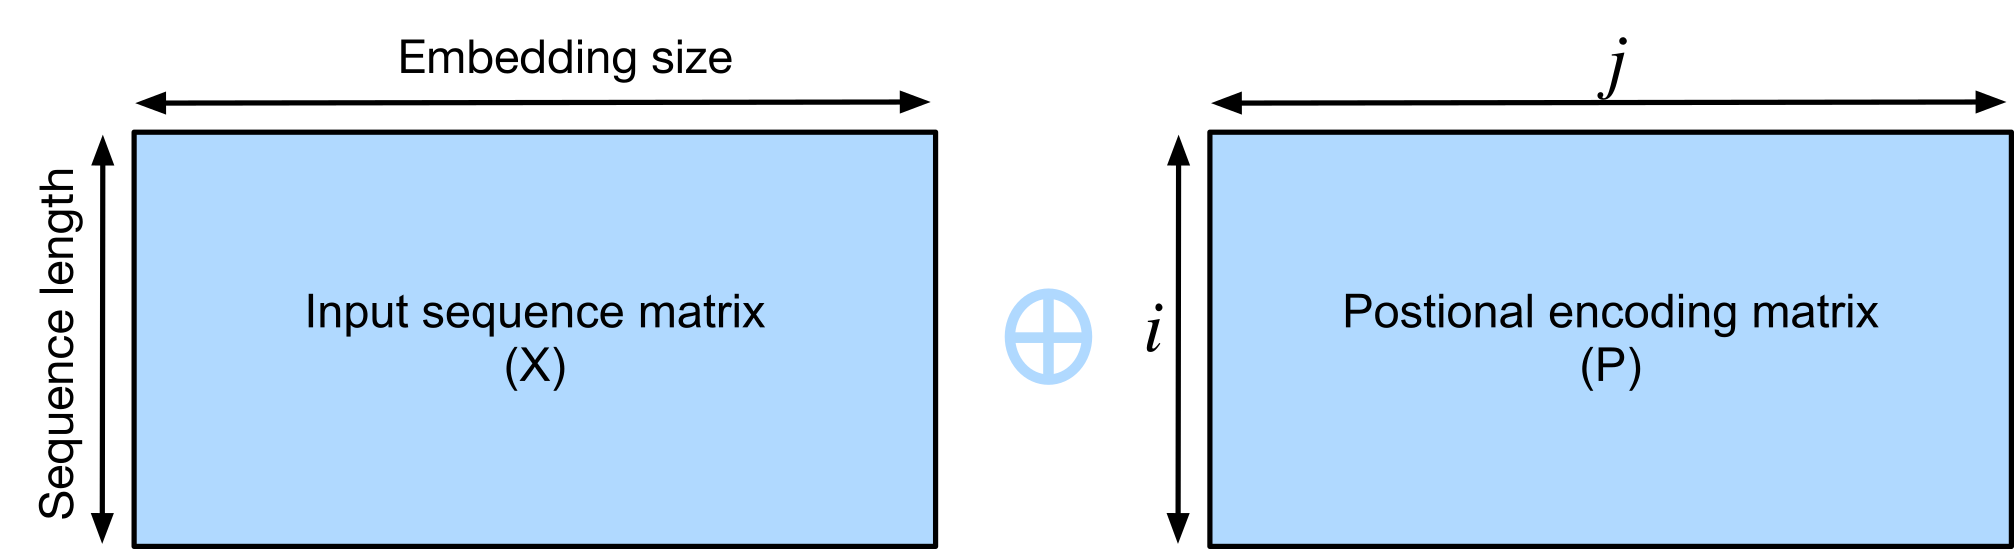
\includegraphics[width=\linewidth]{figures/04-background/positional_encoding.png}
    \caption[Positional encoding]{Positional encoding. Source: \href{https://d2l.ai/chapter_attention-mechanisms/self-attention-and-positional-encoding.html\#positional-encoding}{Dive into Deep Learning}}
    \label{fig:positional_encoding}
\end{figure*}

For a sequence embedding $\vect{Z} \in \reals{l \times d_{\text{model}}}$, the positional encoding matrix $PE \in \reals{l \times d_{\text{model}}}$ is given by:
\begin{align}
    PE_{i,2j} &= \sin{\left( i / 10000^{2j / d_{\text{model}}}  \right)} \\
    PE_{i,2j+1} &= \cos{\left( i / 10000^{2j / d_{\text{model}}}  \right)},
\end{align}

for $i = 1, 2, \dots, l$ and $j = 1, 2, \dots, \floor{d_{\text{model}} / 2}$, where $\floor{\cdot}$ denotes rounding down to the nearest integer.

While \citet{vaswani2017attention} use fixed positional encodings in their work, it is also possible to use learned positional encodings instead \citep{devlin2018bert}.



\section{BERT}
\label{sec:bert}
\glsreset{bert}
A little over two years ago, \citet{devlin2018bert} introduced their new language representation \gls{nn} \gls{bert}.

\gls{bert} is a Transformer-based architecture that uses (only) the \emph{Encoder} stack of the Transformer architecture \citep{vaswani2017attention}, unlike OpenAI's \gls{gpt} and \gls{gpt}-2 networks \citep{radford2018improving,radford2019language}, which use (only) the \emph{Decoder} stack instead, for example. The latter networks use a \gls{lm} objective during pre-training, which involves predicting the next token in a sequence of tokens. This objective requires that these networks are unidirectional, however, such that when computing the self-attention for every token in the sequence, it can only attend to previous tokens. Otherwise the \gls{nn} would learn that the prediction target is the next token in the sequence, which it would then always correctly predict, instead of learning any syntax, grammar or semantics. This unidirectionality requirement significantly limits the choice of architecture.

\subsection{Pre-training Objectives}
\subsubsection{Masked Language Model}
To address the unidirectionality constraint, \citet{devlin2018bert} use a \gls{mlm} objective during pre-training instead. With this objective, some of the tokens in the sequence are randomly masked out and the goal is to predict the original tokens, based only on the context. This objective allows for using both the left and right context, thereby enabling the pre-training of a deep bidirectional Transformer-based \gls{nn}. 

Specifically, \SI{15}{\percent} of the tokens in each sequence are randomly chosen to need a prediction. Of these tokens, \SI{80}{\percent} will be actually masked out with the \texttt{[MASK]} token, \SI{10}{\percent} will be replaced with a random token and \SI{10}{\percent} will remain unchanged. The reasoning by \citet{devlin2018bert} for not always replacing the ``masked'' word with the \texttt{[MASK]} token is that the \texttt{[MASK]} does not appear during the fine-tuning stage, resulting in a mismatch between pre-training and fine-tuning.

\subsubsection{Next Sentence Prediction}
In addition to the \gls{mlm} objective, a \gls{nsp} objective is used to jointly pre-train text-pair representations, which is useful for many down-stream tasks that are based on the relationship between two sentences, like \gls{qa} and \gls{nli}, for example. Specifically, for each pre-training example, \SI{50}{\percent} of the time, sentence \texttt{B} is the actual next sentence that follows sentence \texttt{A}, which is labeled as \texttt{IsNext}. The other \SI{50}{\percent} of the time, sentence \texttt{B} is randomly chosen sentence from the training corpus, which is labeled as \texttt{NotNext}.

\subsubsection{Data}
For their pre-training corpus, \citet{devlin2018bert} use a concatenation of the \gls{tbc} and English Wikipedia (see \cref{subsec:data}). This results in a corpus of roughly \SI{3.3}{\billion} words in total.


\subsection{Input Representations}

BERT uses an input representation that is able to represent both single sentences and sentence pairs, both of which are called a \emph{sequence}. To this end, WordPiece token embeddings \citep{wu2016google} with a vocabulary size of 30522 tokens are used to encode every word in the sequence. The first token of every sequence is always the classification token \cls. 

Furthermore, sentence pairs are packed together into a single sequence, which are differentiated both by the \sep token in between the two sentences, but also by the use of segment embeddings, indicating whether a token belongs to sentence \texttt{A} or sentence \texttt{B}.

Finally, the representation of any input sequence is given by the sum of the token embeddings, segment embeddings and the learned positional encoding, as illustrated in \cref{fig:bert_input}.

\begin{figure*}[ht!]
    \centering
    % \def\svgwidth{0.9\linewidth}
    \def\svgscale{0.8}
    \includesvg{figures/04-background/bert-input}
    % 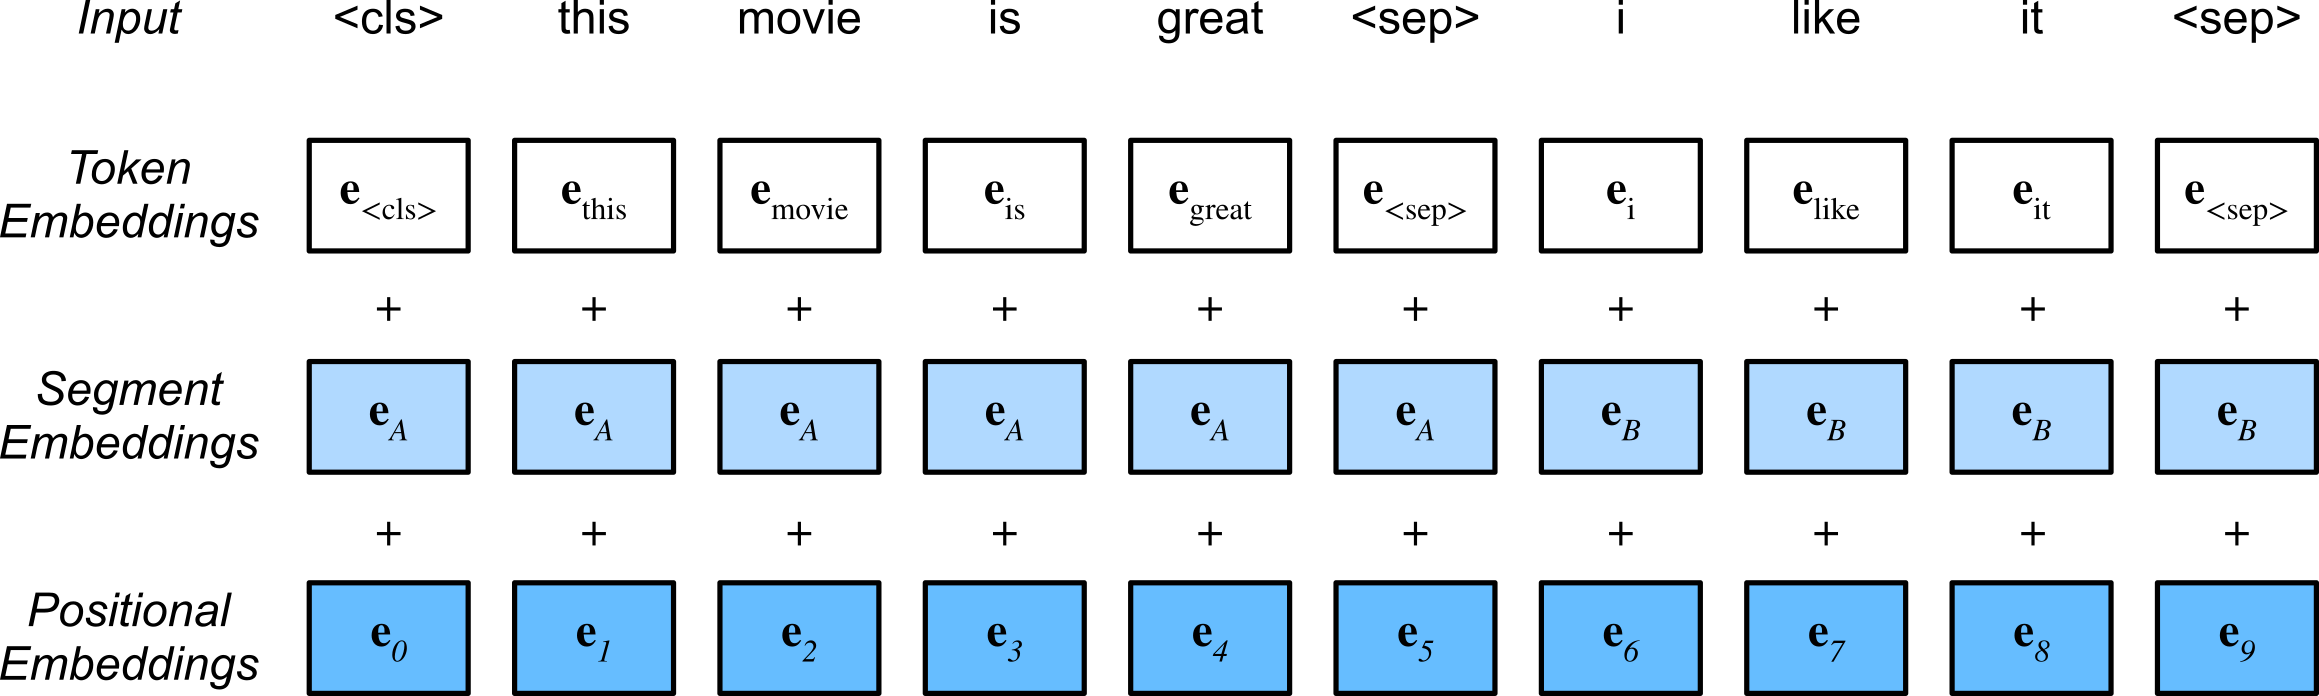
\includegraphics[width=\linewidth]{figures/04-background/bert-input.png}
    \caption[BERT input representation]{The representation of an input sequence for BERT is the sum of the token embeddings, segment embeddings, and positional embeddings. Source: \href{https://d2l.ai/chapter_natural-language-processing-pretraining/bert.html\#input-representation}{Dive into Deep Learning}}
    \label{fig:bert_input}
\end{figure*}

\subsection{Architecture}
\citet{devlin2018bert} use a multi-layer bidirectional Transformer encoder for their network architecture. Furthermore, they present two network sizes, as defined by their number of layers $L$ ($N$ in \citet{vaswani2017attention}), hidden size $H$ ($d_{\text{model}}$) and number of self-attention heads $A$ ($h$).

For both network sizes, a feed-forward size of $4H$ is used, which we will refer to as $FF$ in this work ($d_{ff}$ in \citet{vaswani2017attention}). Lastly, in this work we denote the (total) number of parameters of a particular \gls{nn} as $\#P$. As such, the two network sizes as presented in \citet{devlin2018bert} can be represented as follows:
\begin{enumerate}
    \item \bertbase ($L=12$, $H=768$, $FF=3072$, $A=12$, $\#P=\SI{110}{\mega\nothing}$)
    \item \bertlarge ($L=24$, $H=1024$, $FF=4096$, $A=16$, $\#P=\SI{340}{\mega\nothing}$)
\end{enumerate}

The former network size is used in the present research as our Transformer-based architecture of choice, as mentioned previously.



\section{Knowledge Distillation}
\label{sec:knowledge_distillation}
\glsreset{kd}
Generally speaking, in the context of \glspl{nn}, compression is an umbrella term that covers methods that reduce the size-on-disk, methods that reduce the memory footprint, and methods that increase the computational efficiency of an \gls{nn} (or a combination of these three).  Research into such methods has a long history with early, pioneering works dating back to the late 1980s \citep{janowsky1989pruning,mozer1989skeletonization} and early 1990's \citep{lecun1990optimal,hassibi1993second}. 

Since then, many different techniques have been proposed to make \glspl{nn} more efficient, which can generally be categorized into three categories: \emph{Pruning}, \emph{Quantization} and \gls{kd}\sidenote{More recently, a new, fourth category of \gls{nn} compression techniques has been proposed, called \emph{Theseus Compression} \citep{xu2020bert}, named after the famous thought experiment.}, the last of which is the focus of this section (and more generally: this thesis).

% \subsection{Pruning}
% \label{subsec:pruning}
% \emph{Pruning} is an \gls{nn} compression technique that induces \emph{sparsity}. Sparsity is a measure of how many elements in a tensor are exact zeros, relative to the size of the tensor. For a tensor $\vect{T}$, this is given by the $\ell_0$-``norm''\sidenote{The $\ell_0$-``norm'' used here is not an actual norm, as it is not homogeneous.} of $\vect{T}$, divided by its size:
% \begin{align}
%     \text{sparsity}(\vect{T}) &= \frac{\ell_0\left( \vect{T} \right)}{\left| \vect{T} \right|}, \\
%     \text{where } \ell_0\left( \vect{T} \right) &= \sum_{i=1}^{\left| \vect{T} \right|} \left| \vect{T}_i \right|^0, \nonumber \\
%     \text{and } 0^0 &= 0 \nonumber.
% \end{align}

% \begin{marginfigure}
%     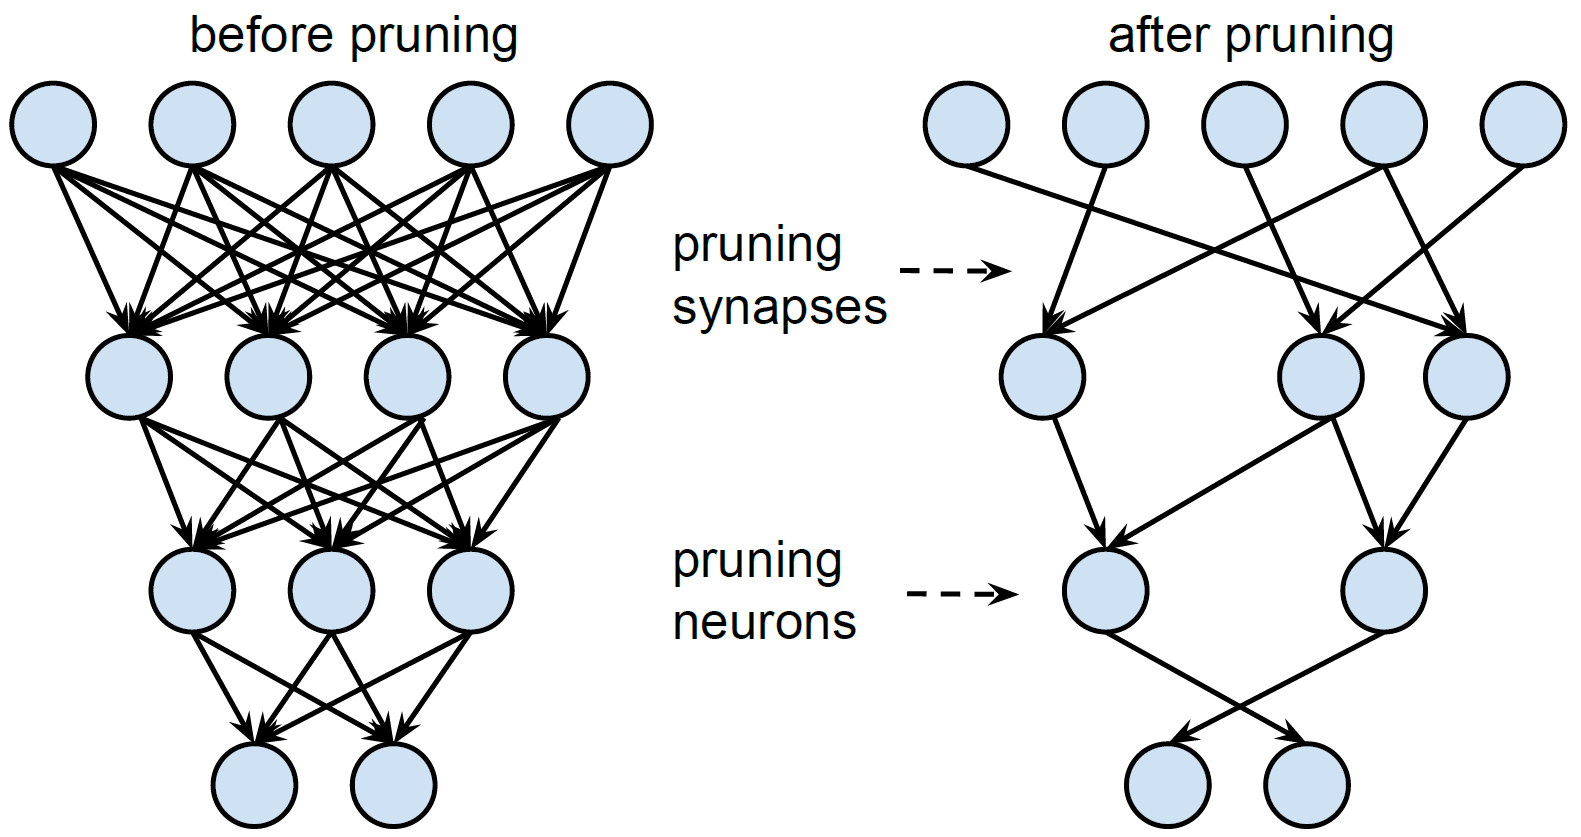
\includegraphics[width=\linewidth]{figures/04-background/pruning.png}
%     \caption[Pruning.]{An \gls{nn} before and after pruning. Source: \citep{han2015learning}}
%     \label{fig:pruning}
% \end{marginfigure}

% With pruning, sparsity is induced by removing weights from an \gls{nn} (setting their value to $0$) based on some criteria (often called ``importance'' or ``saliency''), as illustrated in \cref{fig:pruning}. This makes the \gls{nn} significantly more efficient, albeit at some small cost in terms of accuracy.

% The motivation behind pruning is that often-times \glspl{nn} are over-parameterized and thus contain redundant parameters (i.e. weights). These weights can be safely removed without harming accuracy. This motivation also lies at the core of the \emph{lottery ticket hypothesis} \citep{frankle2018lottery}.

% \paragraph{Magnitude pruning}
% Generally speaking, pruning techniques are differentiated by the criteria they use for selecting the weights that need to be removed. The most widely used method of pruning is called \emph{magnitude pruning}, as introduced by \citet{janowsky1989pruning} and popularized by \citet{han2015learning}.

% With this method, the absolute value of a weight (i.e. its magnitude) is used as the selection criteria, such that it is compared with a certain \emph{threshold value}, and if it is below the threshold, the weight is pruned.

% The motivation for this method is that weights with a small magnitude contribute little to the final prediction (low saliency), making them less important, and therefore best suited for pruning.

% \paragraph{Movement pruning}
% While magnitude pruning is a highly effective, proven method for ``standard'' supervised learning, it proves less suitable in a transfer learning set-up, however. With standard supervised learning, the weight values are determined by the training data of the end-task at hand, whereas with transfer learning, the weight values are predetermined mostly by the original model, and are only fine-tuned on the end-task \citep{sanh2020movement}. 

% To this end, \citet{sanh2020movement} introduced \emph{movement pruning}, which select weights to be pruned based on the \emph{changes} in weight values during fine-tuning. This allows for weights with both small and large (absolute) values to be pruned if they shrink during fine-tuning, thereby leveraging important first-order information.



% \subsection{Quantization}
% \label{subsec:quantization}
% The predominant number format in the context of \glspl{nn} is \gls{fp32}, where any parameter of the \gls{nn} is represented using 32 bits in memory.\sidenote{For example, the number $0.15625$ is represented as $00111110001000000000000000000000$ in memory using \gls{fp32}.} While \gls{fp32} is highly versatile because of its high range and precision, it comes at a significant cost in terms of bandwidth, especially as the number of parameters in an \gls{nn} increases. 

% This is precisely the motivation behind \emph{quantization}, a class of compression methods that rely on reducing the numerical precision of the weights, biases, activations and/or gradients of a neural network.

% \paragraph{Binary quantization}
% Given a weight matrix $\vect{W} \in \reals{m \times n}$, the simplest (and most extreme) quantization method is \emph{binary quantization}, where every weight $W_{i,j}$ is reduced to its sign \citep{gong2014compressing}:
% \begin{align}
%     \hat{\vect{W}}_{i,j} &= \text{sign}(\vect{W}_{i,j}) =  \begin{cases}1 & \text{if } \vect{W}_{i,j} \geq 0, \\ -1 & \text{otherwise}.\end{cases}
% \end{align}

% This method reduces any higher bit-width number to a single bit. In the case of \gls{fp32}, for example, this yields a compression ratio of $32 \times$.

% \paragraph{$N$-bit Quantization}
% While binary quantization yields a high compression ratio, it might be too crude for the task at hand, resulting in a significantly worse accuracy. As such, a higher bit-width of $N$-bits might be preferred. Generalizing binary ($1$-bit) quantization to $N$-bit quantization is straightforward:
% \begin{align}
%     \hat{\vect{W}}_{i,j} &= \text{clip}\left( \round{\frac{\vect{W}_{i,j}}{N}} N, -M, M \right), \\
%     \text{where } \text{clip}\left( x, a, b \right) &= \min{(\max{(x, a)}, b)}, \nonumber \\
%     \text{and } M &= 2^{N-1} - 1, \nonumber
% \end{align}

% and $\round{\cdot}$ denotes rounding to the nearest integer \citep{hubara2017quantized}. This method would yield a compression ratio of $\frac{32}{N} \times$.

\gls{kd} as introduced by \citet{bucil2006model}, and popularized by \citet{hinton2015distilling}, is a \gls{nn} compression method in which a smaller (untrained) student network is trained to mimic a larger, (pre-)trained teacher network or ensemble of teacher networks by means of \emph{knowledge transfer}. More formally, the student network is trained on some transfer dataset $\dataset_T$ to minimize a loss function in which the target is the distribution of class probabilities as output by the teacher network (``soft target loss'' or ``distillation loss''):
\begin{align}
    \label{eq:soft_target_loss}
    \loss{\vect{z}_s, \vect{z}_t} &= KL\left( \softmax{\vect{z}_s} || \softmax{\vect{z}_t} \right),
\end{align}

where $\vect{z}_s$ and $\vect{z}_t$ are the student and teacher logits (i.e. the raw, unnormalized predictions by the \gls{nn}), respectively, $\softmax{\cdot}$ is the softmax function, and $KL(p || q)$ is the \gls{kld}.

Not only does this soft target loss allow for the data in $\dataset_T$ to be entirely unlabeled, but it also provides a richer signal during training when compared to only using the ground truth label as your target.

A well-trained teacher network, however, often-times predicts the ``true'' class (ground truth label) at a (very) high probability, while the other class probabilities are close to $0$. This would make the signal no more informative than the ground truth label itself. To address this issue, \citet{hinton2015distilling} use a \emph{temperature} $T > 1$ in the softmax function (during training) in order to yield a softer probability distribution over the classes:

\begin{align}
    \label{eq:soft_target_loss_scaled}
    \mathcal{L}_{\text{soft}} = \loss{\vect{z}_s, \vect{z}_t} &= KL\left( \softmax{\vect{z}_s / T} || \softmax{\vect{z}_t / T} \right).
\end{align}

When some or all of the data in $\dataset_T$ is labeled, \citet{hinton2015distilling} have found it beneficial, in addition to the soft target loss, to train the student network to also predict the ground truth labels $\vect{y}$ (``hard target loss'' or ``student loss''):
\begin{align}
    \label{eq:hard_target_loss}
    \mathcal{L}_{\text{hard}} = \loss{\vect{z}_s, \vect{y}} &= \ce{\softmax{\vect{z}_s}, \vect{y}},
\end{align}

where $\ce{\softmax{\vect{z}_s}, \vect{y}}$ is the \gls{ce} between the class probability distribution of the student network and the ground truth labels. Combining the loss functions defined in \cref{eq:soft_target_loss_scaled,eq:hard_target_loss} yields the following combined loss function:
 
\begin{align}
    \label{eq:combined_kd_loss}
    \mathcal{L}_{\text{combined}} &= \loss{\vect{z}_s, \vect{z}_t, \vect{y}}, \nonumber \\
    &= \alpha \cdot T^2 \cdot KL\left( \softmax{\vect{z}_s / T} || \softmax{\vect{z}_t / T} \right) \nonumber \\
    &\quad + \beta \cdot \ce{\softmax{\vect{z}_s}, \vect{y}},  
\end{align}

where $\alpha$ and $\beta$ are coefficients. When using a combination of both soft and hard targets, it is important to multiply the soft target loss by $T^2$, as the magnitude of its gradient scales as $1/T^2$. Furthermore, in their work, \citet{hinton2015distilling} found it better to use a simple weighted average of the two objective functions. Practically this means: $\alpha = 0.5$, and $\beta = 1 - \alpha = 0.5$.



\section{Evaluation}
\label{sec:evaluation}
\glsreset{glue}
\glsreset{squad}
In the context of \gls{nlu}, certain evaluation methods have significantly risen in popularity in recent years, to the point where one could consider them a ``standard''. Doing our best not to reinvent the wheel, this work follows the good example set by those before us (see \cref{ch:related_work}), and uses these ``standard'' evaluation methods to verify the validity of our approach and compare our approach to others.

To this end, this section first details the \gls{glue} benchmark in \cref{subsec:GLUE}, before introducing the \gls{squad} in \cref{subsec:SQuAD}.


\subsection{GLUE}
\label{subsec:GLUE}
The \gls{glue} benchmark \citep{wang2018glue} is a diverse collection of 9 \gls{nlu} tasks (with accompanying datasets) spanning 3 different categories: single-sentence tasks, similarity and paraphrase tasks, and inference tasks.\sidenote{The GLUE leaderboard can be found here: \href{https://gluebenchmark.com/leaderboard}{https://gluebenchmark.com/leaderboard}} The goal of the benchmark is to assess how well a \gls{nn} is able to generalize when it comes to \gls{nlu} (i.e. good performance on the benchmark requires shared knowledge between the different tasks).

A brief description and some relevant statistics of all tasks included in \gls{glue} are presented in \cref{tab:glue_datasets}, before providing a more detailed description of each task below.

\begin{table*}[ht]
    \footnotesize
    \centering
    \begin{tabular}{l|r|r|l|l}
        \toprule
        \B{Dataset} & \B{$\sizeof{\text{Train}}$} & \B{$\sizeof{\text{Test}}$} & \B{Task} & \B{Metric(s)} \\
        \midrule
        \multicolumn{5}{c}{Single-sentence tasks} \\
        \midrule
        CoLA & \SI{3.7}{\kilo\nothing} & \SI{1.7}{\kilo\nothing} & acceptability & Matthews correlation coefficient \\
        SST-2 & \SI{67}{\kilo\nothing} & \SI{1.8}{\kilo\nothing} & sentiment & accuracy \\
        \midrule
        \multicolumn{5}{c}{Similarity and paraphrase tasks} \\
        \midrule
        MRPC & \SI{3.7}{\kilo\nothing} & \SI{1.7}{\kilo\nothing} & paraphrase & accuracy/ F$_{\text{1}}$ score \\
        QQP & \SI{364}{\kilo\nothing} & \SI{391}{\kilo\nothing} & paraphrase & accuracy/ F$_{\text{1}}$ score \\
        STS-B & \SI{7}{\kilo\nothing} & \SI{1.4}{\kilo\nothing} & sentence similarity & Pearson/Spearman correlation coefficients \\
        \midrule
        \multicolumn{5}{c}{Inference tasks} \\
        \midrule
        MNLI & \SI{393}{\kilo\nothing} & \SI{20}{\kilo\nothing} & \gls{nli} & matched accuracy / mismatched accuracy\\
        QNLI & \SI{105}{\kilo\nothing} & \SI{5.4}{\kilo\nothing} & \gls{qa} / \gls{nli} & accuracy \\
        RTE & \SI{2.5}{\kilo\nothing} & \SI{3}{\kilo\nothing} & \gls{nli} & accuracy \\
        WNLI & \num{634} & \num{146} & coreference / \gls{nli} & accuracy \\
        \bottomrule
    \end{tabular}
    \caption[GLUE dataset descriptions and statistics][0.5cm]{Descriptions and statistics for all 9 tasks included in the GLUE benchmark. Almost all tasks are binary classification tasks, except for STS-B, which is a regression task, and MNLI, which uses 3 classes. Adapted from \citet{wang2018glue}.}
    \label{tab:glue_datasets}
\end{table*}

\subsubsection{Single-sentence tasks}
\paragraph{CoLA}
The \gls{cola} \citep{warstadt2019neural} is a binary classification task, where each sentence is classified as either a grammatical English sentence or not (linguistic acceptability). The sentences were drawn from books and articles on linguistic theory. Performance is evaluated by means of the Matthews correlation coefficient \citep{matthews1975comparison}, which gives a score in $\intervalcc{-1, 1}$, where $0$ would be akin to random guessing.

\paragraph{SST-2}
The \gls{sst} \citep{socher2013recursive} is also a binary classification task, where each sentence is classified as either positive or negative (sentiment analysis). The sentences were drawn from movie reviews, with human annotations of their sentiment. Simple classification accuracy is used for evaluation.

\subsubsection{Similarity and paraphrase tasks}
\paragraph{MRPC}
The \gls{mrpc} \citep{dolan2005automatically} consists of sentence pairs extracted from online news sources (automatically), with human annotations of whether the sentences are semantically equivalent or not. As the classes are imbalanced (\SI{68}{\percent} positive), both accuracy and F$_{\text{1}}$ score are used to measure performance.

\paragraph{QQP}
\gls{qqp} \citep{iyer2018quora} consists of sentence pairs drawn from the popular community \gls{qa} website \href{https://www.quora.com}{Quora}, where each sentence pair is classified to be semantically equivalent or not. Similar to MRPC, due to class imbalance (\SI{37}{\percent} positive), both accuracy and F$_{\text{1}}$ score are used to measure performance.

\paragraph{STS-B}
The \gls{stsb} \citep{cer2017semeval} is a regression task, where each sentence pair is classified using scores in $\intervalcc{0, 5}$ to denote their similarity in terms of semantics, where a score of $0$ would mean that the two sentences are completely dissimilar and a score of $5$ would mean that the two sentences are completely equivalent. The sentence pairs were drawn from news headlines and other sources, with human annotations for their semantic similarity. Performance is measured by means of Pearson and Spearman correlation coefficients.


\subsubsection{Inference tasks}
\label{subsubsec:inference_tasks}
\paragraph{MNLI}
\gls{mnli} \citep{williams2017broad} is a textual entailment classification task, where the goal for each sentence pair is to predict whether the first sentence (\emph{premise}) entails the second sentence (\emph{hypothesis}), contradicts it or neither. As such, this is a ternary classification task with \emph{entailment}, \emph{contradiction}, and \emph{neutral} as its labels. The sentence pairs were collected from ten different genres of written and spoken English, such as face-to-face conversations, political speeches, letters, magazine articles, works of fictions, etc. The task actually contains two \emph{sections}: a \emph{matched} section, where the genre of the sentence pairs in the train set match with those in the test set, and a \emph{mismatched} section, where the sentence pairs of the train and test set are of different genres. Performance is measured by accuracy on the matched and mismatched sections (separately).

\paragraph{QNLI}
\gls{qnli} is a recasting of the SQuAD dataset (see \cref{subsec:SQuAD}), where for each question-paragraph pair, question-sentence pairs are formed between the question and each sentence in the paragraph with enough lexical overlap. The task is to classify whether the paragraph sentence contains the answer to the question. Performance is measured using simple classification accuracy.

\paragraph{RTE}
\gls{rte} is another recasting of existing datasets, where the authors combine the data from RTE1 \citep{dagan2005pascal}, RTE2 \citep{haim2006second}, RTE3 \citep{giampiccolo2007third} and RTE5 \citep{bentivogli2009fifth} into a single dataset. The dataset consists of sentence pairs with binary textual entailment labels\sidenote{For RTE5, \texttt{UNKNOWN} and \texttt{CONTRADICTION} are collapsed to \texttt{NOT\_ENTAILMENT} for consistency.}. Classification accuracy is used to evaluate performance.

\paragraph{WNLI}
\label{par:wnli}
\gls{wnli} consists of sentence pairs, where the first sentence (\emph{premise}) contains an ambiguous pronoun and the second sentence contains a possible referent (\emph{hypothesis}). The task is to predict whether the first sentence entails the second. The sentence pairs were constructed from the Winograd Schema Challenge dataset \citep{levesque2012winograd}, which consists of sentences with ambiguous pronouns and a list of possible referents of that pronoun. Performance is measured using classification accuracy.\sidenote{The authors note that this task has an adversarial development set (examples in the development set sometimes share its hypothesis with an example in the training set), and an imbalanced test set (\SI{65}{\percent} not entailment), both of which could yield unexpected (negative) results.}


\subsection{SQuAD}
\label{subsec:SQuAD}
\gls{squad} (v1.1) \citep{rajpurkar2016squad} is a sizable reading comprehension dataset with more than 100k crowd-sourced question-passage pairs\sidenote{The passages were sourced from articles of English Wikipedia.}, where the passage contains the answer to the question\sidenote{Actually, the passage might contain more than one possible answer to the specific question, as we will see in the example provided below.}, and the task is to predict the span of text in the passage that contains this answer.\sidenote{The SQuAD leaderboard can be found here: \href{https://rajpurkar.github.io/SQuAD-explorer/}{https://rajpurkar.github.io/SQuAD-explorer/}} 

Performance is measured using two metrics, which both ignore punctuation marks and articles (e.g. ``an'', ``the'', etc.):

\paragraph{Exact Match}
The \gls{em} metric is measured by the number of predictions that match the ground truth answer(s) \emph{exactly}, as a percentage of the total number of predictions.


\paragraph{(Macro-averaged) F$_{\text{1}}$ score} In the context of \gls{squad}, for a specific question, the F$_{\text{1}}$ score is computed using the \gls{bot}\sidenote{Analogues to \gls{bow}, but then for tokens.} representation of both the predicted answer and the ground truth answer. If a question contains multiple ground truth answers, the F$_{\text{1}}$ score for that question is given by the maximum F$_{\text{1}}$ score over all the ground truth answers. These F$_{\text{1}}$ scores for all questions are averaged in order to obtain the macro-average F$_{\text{1}}$ score.

An example from the development set of \gls{squad} is given below, where the different ground truth answers have been color-coded for the convenience of the reader:

\begin{fullwidth}
    \noindent
    \small
    \begin{tabular}{p{0.25\linewidth} p{0.75\linewidth}}
        \B{Passage:} & \I{Super Bowl 50 was an American football game to determine the champion of the National Football League (NFL) for the 2015 season. The American Football Conference (AFC) champion Denver Broncos defeated the National Football Conference (NFC) champion Carolina Panthers 24–10 to earn their third Super Bowl title. The game was played on February 7, 2016, at \textcolor{pink}{\hl{Levi's Stadium}}\hl{ in the San Francisco Bay Area at }\textcolor{indigo}{\hl{Santa Clara, California}}. As this was the 50th Super Bowl, the league emphasized the "golden anniversary" with various gold-themed initiatives, as well as temporarily suspending the tradition of naming each Super Bowl game with Roman numerals (under which the game would have been known as "Super Bowl L"), so that the logo could prominently feature the Arabic numerals 50.} \\ \addlinespace
        \B{Question:} & Where did Super Bowl 50 take place? \\ \addlinespace
        \B{Ground truth answer(s):} & \textcolor{pink}{Levi's Stadium} \\ 
        & \textcolor{indigo}{Santa Clara, California} \\ 
        & \hl{Levi's Stadium in the San Francisco Bay Area at Santa Clara, California}
    \end{tabular}
\end{fullwidth}
